\section{Ranking queries}

Ranking queries, also called top-$k$ queries, aim to retrieve only the $k$ best ansoftwareers from a potentially very large result set. Ranking is based on ordering objects based on their relevance.

Assume a scoring function $S$ that assigns to each tuple $t$ a numerical score for ranking tuples. The algorithm needs these inputs: cardinality $k$, dataset $R$, and a scoring function $S$. The output is 
the $k$ highest-scored tuples with respect to $S$. The idea is the following: 
\begin{enumerate}
    \item For all tuples $t$ in $R$ compute $S(t)$. 
    \item Sort tuples based on their scores.
    \item Return the first $k$ highest-scored tuples. 
\end{enumerate}
This naïve approach is expensive for large dataset because it requires to sort a large amount of data. It is even worse if more than one relation is involved because it needs to join all tuples. So, 
we now know that two abilities are required: 
\begin{itemize}
    \item Ordering the tuples according to their scores. This is taken care of by 
        \begin{lstlisting}[style=SQL]
ORDER BY
        \end{lstlisting}
    \item Limiting the output cardinality to $k$ tuples. This is taken care of by 
        \begin{lstlisting}[style=SQL]
FETCH FIRST k ROWS ONLY
        \end{lstlisting}
\end{itemize} 
\begin{example}
    Consider the following queries: 
    \begin{lstlisting}[style=SQL]
a)  SELECT *
FROM UsedCarsTable
WHERE Vehicle = 'Audi/A4'
AND Price <= 21000
ORDER BY 0.8*Price+0.2*Miles
b)  SELECT *
FROM UsedCarsTable
WHERE Vehicle = 'Audi/A4'
ORDER BY 0.8*Price+0.2*Miles
    \end{lstlisting}
    The values 0.8 and 0.2, also called weights, are a way to normalize our preferences on price and mileage.
    The first query will likely miss some relevant ansoftwareers (near-miss). The second query will return all Audi/A4 in the dataset (information overload).
\end{example}
Only the first $k$ tuples become part of the result. If more than one set of $k$ tuples satisfies the ordering directive, any of such sets is a valid ansoftwareer 
(non-deterministic semantics). 

To evaluate a top-$k$ query it is possible to consider two basic aspects: 
\begin{itemize}
    \item Query type: one relation, many relations, and aggregate results. 
    \item Access paths: no index, indexes on all/some ranking attributes. 
\end{itemize}
In the simplest case, that is a top-$k$ selection query with only one relation, if the input is sorted according to $S$ it is possible to read only the first $k$ tuples; 
If the tuples are not sorted we need to perform an in-memory sort (through the heap), that has a complexity of $O(N\log{k})$. 
\begin{example}
    Consider the two-dimensional attribute space (Price, Mileage) of the previous example: 
    \begin{figure}[H]
        \centering
        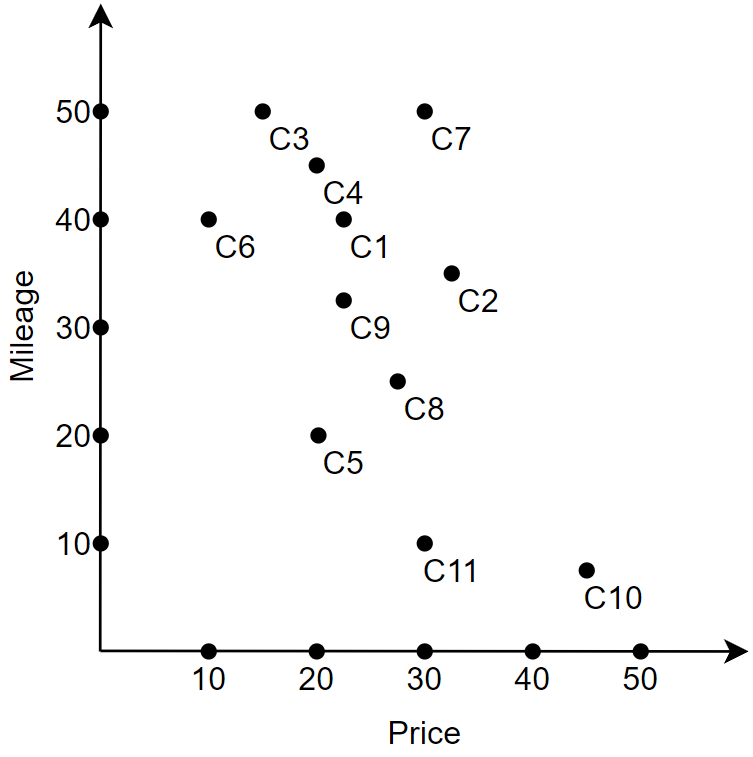
\includegraphics[width=0.25\linewidth]{images/ex1.png}
    \end{figure}
    In the image each tuple is represented by a two-dimensional point $(p, m)$, where $p$ is the Price and $m$ is the Mileage. Intuitively, minimizing
    $0.8\cdot Price + 0.2\cdot Mileage$ is equivalent to looking for points close to $(0,0)$. Our preferences are essential to determine the result. Consider the line of equation: 
    \[0.8\cdot Price + 0.2\cdot Mileage = v\]
    where $v$ is a constant. This can also be written as:
    \[Mileage = -4\cdot Price + 5\cdot v\]
    from which we see that all the lines have a slope $-4$. By definition, all the points of the same line are equally good. If we change the weights, it is possible 
    that the best choice also varies. 
    The target of a query is not necessarily $(0,0)$, rather it can be any point $q=(q_1,q_2)$. 
\end{example}
In general, in order to determine the goodness of a tuple $t$, we compute its distance from the target point $q$: the lower the distance from $q$, the better. 
If we consider the distances the model become: 
\begin{itemize}
    \item An $m$-dimensional $(m \geq 1)$ space $A = (A_1,A_2,\dots,A_m)$ of ranking attributes. 
    \item A relation $R(A_1,A_2,\dots,A_m,B_1,B_2,\dots)$, where $B_1,B_2,\dots$ are other attributes.
    \item A target point $q = (q_1,q_2,\dots,q_m)$, $q \in A$. 
    \item A function $d: A \times A \rightarrow \mathbb{R}^{+}$, measuring the distance between points in $A$. 
\end{itemize}
\begin{definition}
    The top-$k$ query is called $k$-\emph{nearest neighbors} if given a point $q$, a relation $R$, an integer $k \geq 1$, and a distance function $d$ it determines the $k$ tuples 
    in $R$ that are closest to $q$ according to $d$. 

    The distance function called $L_p$-\emph{norms} is defined as:
    \[L_p(t,q)=\left(\sum_{i=1}^{m}{\left\lvert t_i-q_i \right\rvert^{p}}\right)^{\frac{1}{p}}\]
\end{definition}
Relevant cases of the $L_p$-norm are: 
\begin{itemize}
    \item Euclidean distance (ellipsoids): $L_2(t,q)=\sqrt{\sum_{i=1}^{m}{\left\lvert t_i-q_i \right\rvert^{2}}}$
    \item Manhattan distance (rhomboids): $L_1(t,q)=\sum_{i=1}^{m}{\left\lvert t_i-q_i \right\rvert}$
    \item Čebyšëv distance (rectangles): $L_{\infty}(t,q)=\max_{i}\{\left\lvert t_i-q_i\right\rvert\}$
\end{itemize}
The shape of the attribute space depends on the distance function and the weight associated to each coordinate: 
\begin{itemize}
    \item Euclidean distance (hyper-ellipsoids):
        \[L_2(t,q;W)=\sqrt{\sum_{i=1}^{m}{w_i\left\lvert t_i-q_i \right\rvert^{2}}}\]
    \item Manhattan distance (hyper-rhomboids): 
        \[L_1(t,q;W)=\sum_{i=1}^{m}{w_i\left\lvert t_i-q_i \right\rvert}\]
    \item Čebyšëv distance (hyper-rectangles): 
        \[L_{\infty}(t,q;W)=\max_{i}\{w_i \left\lvert t_i-q_i\right\rvert\}\]
\end{itemize}
\begin{definition}
    In a \emph{top-$k$ join query} we have $n > 1$ input relations and a scoring function $S$ defined on the result of the join. The general formula is: 
    \begin{lstlisting}[style=SQL]
SELECT <attributes>
FROM R1,R2,...,Rn
WHERE <conditions>
ORDER BY S(p1,p2,...,pm) [DESC]
FETCH FIRST k ROWS ONLY             
    \end{lstlisting}
    where $p_1,p_2,\dots,p_m$ are the scoring criteria. 
\end{definition}

In the top-$k$ $1-1$ join queries all the joins are on a common key attribute. It is possible to have two main scenarios: 
\begin{itemize}
    \item There is an index for retrieving tuples according to each preference. 
    \item The relation is spread over several sites, each providing information only on part of the objects.
\end{itemize}
We make the following assumptions: 
\begin{itemize}
    \item Each input list supports sorted access: this means that each access returns the identifier of the next best object, its partial score $p_j$. 
    \item Each input list supports random access: this means that each access returns the partial score of an object, given its identifier. 
    \item The identifier of an object is the same across all inputs. 
    \item Each input consists of the same set of objects. 
\end{itemize}
\begin{example}
    Given the following reviews on two different sites: 
    \begin{table}[H]
        \centering
        \begin{tabular}{ccccc}
        \multicolumn{1}{l}{\textbf{EatWell}}     &                                     & $\:\:\:\:\:\:$                 & \multicolumn{1}{l}{\textbf{BreadAndWine}} &                                  \\ \cline{1-2} \cline{4-5} 
        \multicolumn{1}{|l}{\textbf{Name}}       & \multicolumn{1}{c|}{\textbf{Score}} & \multicolumn{1}{c|}{\textbf{}} & \multicolumn{1}{l}{\textbf{Name}}        & \multicolumn{1}{c|}{\textbf{Score}} \\ \cline{1-2} \cline{4-5} 
        \multicolumn{1}{|l}{The old mill}        & \multicolumn{1}{c|}{9.2}            & \multicolumn{1}{c|}{}          & \multicolumn{1}{l}{Da Gino}              & \multicolumn{1}{c|}{9.0}            \\
        \multicolumn{1}{|l}{The canteen}         & \multicolumn{1}{c|}{9.0}            & \multicolumn{1}{c|}{}          & \multicolumn{1}{l}{Cheers!}              & \multicolumn{1}{c|}{8.5}            \\  
        \multicolumn{1}{|l}{Cheers!}             & \multicolumn{1}{c|}{8.3}            & \multicolumn{1}{c|}{}          & \multicolumn{1}{l}{The old mill}         & \multicolumn{1}{c|}{7.5}            \\ 
        \multicolumn{1}{|l}{Da Gino}             & \multicolumn{1}{c|}{7.5}            & \multicolumn{1}{c|}{}          & \multicolumn{1}{l}{Chez Paul}            & \multicolumn{1}{c|}{7.5}            \\ 
        \multicolumn{1}{|l}{Let's eat!}          & \multicolumn{1}{c|}{6.4}            & \multicolumn{1}{c|}{}          & \multicolumn{1}{l}{The canteen}          & \multicolumn{1}{c|}{7.0}            \\ 
        \multicolumn{1}{|l}{Chez Paul}           & \multicolumn{1}{c|}{5.5}            & \multicolumn{1}{c|}{}          & \multicolumn{1}{l}{Los pollos hermanos}  & \multicolumn{1}{c|}{6.5}            \\ 
        \multicolumn{1}{|l}{Los pollos hermanos} & \multicolumn{1}{c|}{5.0}            & \multicolumn{1}{c|}{}          & \multicolumn{1}{l}{Let's eat!}           & \multicolumn{1}{c|}{6.0}            \\ \cline{1-2} \cline{4-5} 
        \end{tabular}
    \end{table}
    If we aggregate the two tables with the following query: 
    \begin{lstlisting}[style=SQL]
SELECT *
FROM EatWell EW, BreadAndWine BW
WHERE EW.Name = BW.Name
ORDER BY EW.Score + BW.Score DESC
FETCH FIRST 1 ROW ONLY 
    \end{lstlisting}
    We will obtain the following result: 
    \begin{table}[H]
        \centering
        \begin{tabular}{|lc|}
        \hline
        \textbf{Name}       & \textbf{Global score} \\ \hline
        Cheers!             & 16.8                  \\ \hline
        The old mill        & 16.7                  \\ \hline
        Da Gino             & 16.5                  \\ \hline
        The canteen         & 16.0                  \\ \hline
        Chez Paul           & 13.0                  \\ \hline
        Let's eat!          & 12.4                  \\ \hline
        Los pollos hermanos & 11.5                  \\ \hline
        \end{tabular}
    \end{table}
    Note that the winner is not the best locally. 
\end{example}
Each object o returned by the input $L_j$ has an associated local/partial score $p_j(o) \in [0,1]$. For convenience, scores are normalized. The hypercube $[0,1]^m$ 
is called the score space. The point $p(o) = (p_1(o),p_2(o),\dots,p_m(o)) \in [0,1]^m$ is the map of $o$ into the score space. The global score $S(o)$ of $o$ is 
computed by means of a scoring function $S$ that combines in some way the local scores of $o$:
\[S(o) \equiv  S(p(o)) = S(p_1(o),p_2(o),\dots,p_m(o))\]
with $S:[0,1]^m \rightarrow \mathbb{R}^{+}$. 
\begin{example}
    Consider the attribute space $A = (Price,Mileage)$
    \begin{figure}[H]
        \centering
        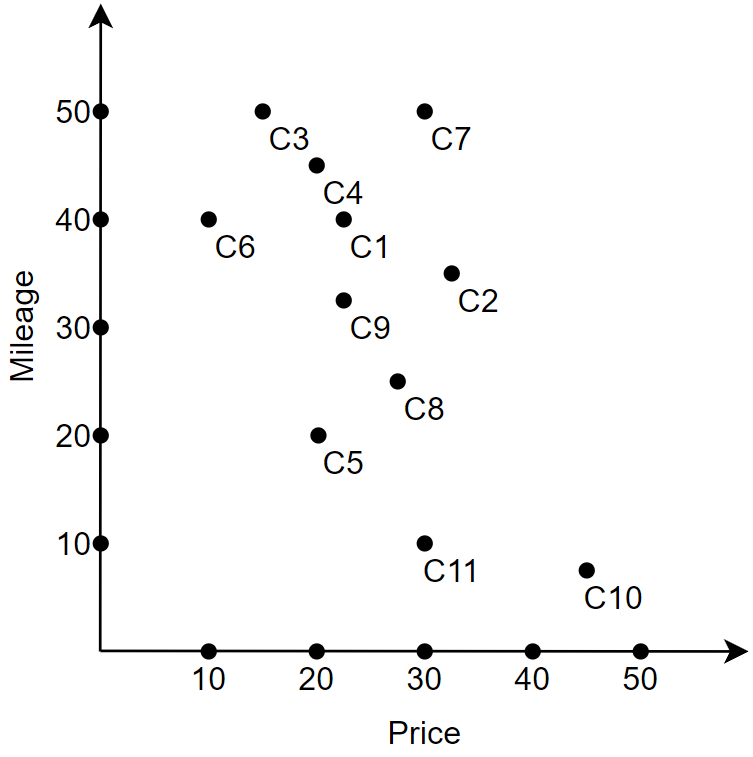
\includegraphics[width=0.25\linewidth]{images/ex1.png}
    \end{figure}
    If we choose $MaxP = 50,000$ and $MaxM = 80,000$, we have that a generic point $o$ is mapped with these formulas: 
    \[p_1(o) = 1 - \dfrac{o.Price}{MaxP} \:\:\:\:\:\: p_2(o) = 1 - \dfrac{o.Mileage}{MaxM}\]
    Graphically we have; 
    \begin{figure}[H]
        \centering
        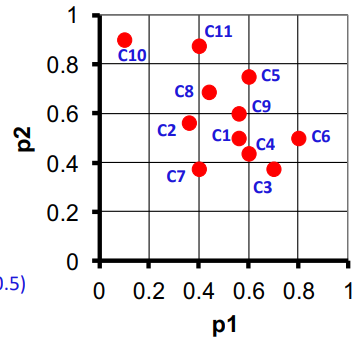
\includegraphics[width=0.3\linewidth]{images/ex2.png}
    \end{figure}
\end{example}
The most common scoring functions are: 
\begin{itemize}
    \item Average (SUM), that weighs preferences equally
        \[\textnormal{SUM}(o) \equiv \textnormal{SUM}(p(o)) = p_1(o) + p_2(o) + \dots + p_m(o)\]
    \item Weighted sum (WSUM), that weighs the preferences differently
        \[\textnormal{WSUM}(o) \equiv \textnormal{WSUM}(p(o)) = w_1p_1(o) + w_2p_2(o) + \dots + w_mp_m(o)\]
    \item Minimum (MIN), that considers the worst partial score
        \[\textnormal{MIN}(o) \equiv \textnormal{MIN}(p(o)) = \min\{p_1(o),p_2(o),\dots, p_m(o)\}\]
    \item Maximum (MAX), that considers the best partial score
        \[\textnormal{MAX}(o) \equiv \textnormal{MAX}(p(o)) = \max\{p_1(o),p_2(o),\dots, p_m(o)\}\]       
\end{itemize}
Note that even with the minimum scoring function we always want to retrieve the $k$ objects with the highest global scores.

It is possible to define e iso-score curves in the score space, which are set of points with the same global score. 
\begin{example}
    In the previous graph we have that the iso-score curves for the maximum function are: 
    \begin{figure}[H]
        \centering
        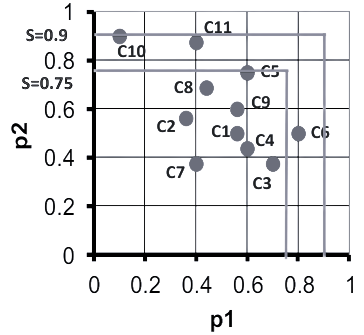
\includegraphics[width=0.3\linewidth]{images/iso.png}
    \end{figure}
    In the previous graph we have that the iso-score curves for the minimum function are: 
    \begin{figure}[H]
        \centering
        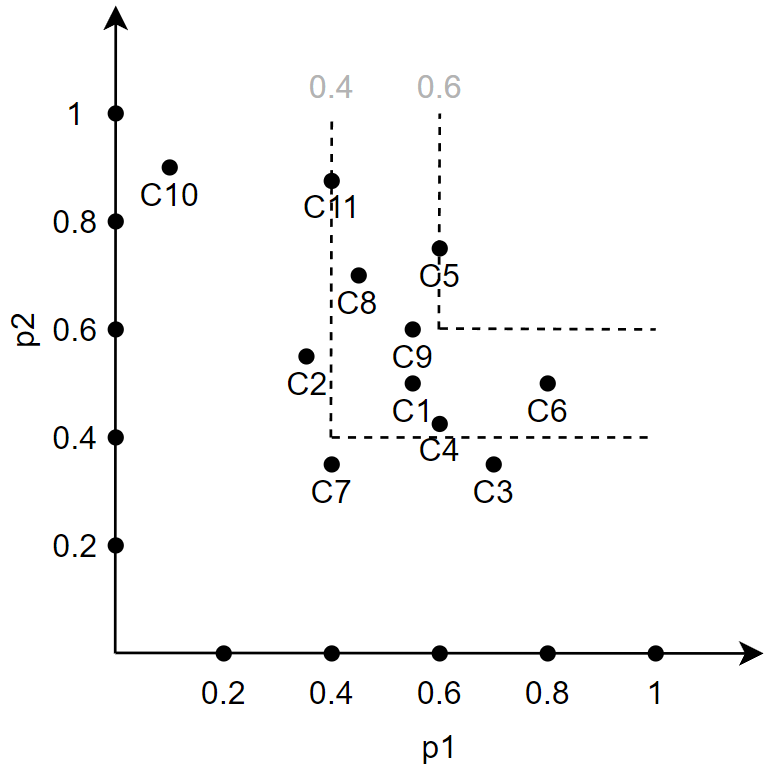
\includegraphics[width=0.3\linewidth]{images/isomin.png}
    \end{figure}
\end{example}

\subsection*{B-zero algorithm}
It is possible to efficiently compute the result of a top-k 1-1 join query using a maximum scoring function $S$ using the $B_0$ algorithm. The inputs
of this algorithm are: an integer $k \geq 1$, and a ranked list $R_1,\dots,R_m$. The idea is: 
\begin{enumerate}
    \item Make $k$ sorted accesses on each list and store objects and partial scores in a buffer $B$. 
    \item For each object in $B$, compute the MAX of its (available) partial scores.
    \item Return the $k$ objects with maximum score.
\end{enumerate}
This algorithm is instance-optimal. 
\begin{example}
    Given the following reviews on two different sites: 
    \begin{table}[H]
        \centering
        \begin{tabular}{ccccc}
        \multicolumn{1}{l}{\textbf{EatWell}}     &                                     & $\:\:\:\:\:\:$                 & \multicolumn{1}{l}{\textbf{BreadAndWine}} &                                  \\ \cline{1-2} \cline{4-5} 
        \multicolumn{1}{|l}{\textbf{Name}}       & \multicolumn{1}{c|}{\textbf{Score}} & \multicolumn{1}{c|}{\textbf{}} & \multicolumn{1}{l}{\textbf{Name}}        & \multicolumn{1}{c|}{\textbf{Score}} \\ \cline{1-2} \cline{4-5} 
        \multicolumn{1}{|l}{The old mill}        & \multicolumn{1}{c|}{9.2}            & \multicolumn{1}{c|}{}          & \multicolumn{1}{l}{Da Gino}              & \multicolumn{1}{c|}{9.0}            \\
        \multicolumn{1}{|l}{The canteen}         & \multicolumn{1}{c|}{9.0}            & \multicolumn{1}{c|}{}          & \multicolumn{1}{l}{Cheers!}              & \multicolumn{1}{c|}{8.5}            \\  
        \multicolumn{1}{|l}{Cheers!}             & \multicolumn{1}{c|}{8.3}            & \multicolumn{1}{c|}{}          & \multicolumn{1}{l}{The old mill}         & \multicolumn{1}{c|}{7.5}            \\ 
        \multicolumn{1}{|l}{Da Gino}             & \multicolumn{1}{c|}{7.5}            & \multicolumn{1}{c|}{}          & \multicolumn{1}{l}{Chez Paul}            & \multicolumn{1}{c|}{7.5}            \\ 
        \multicolumn{1}{|l}{Let's eat!}          & \multicolumn{1}{c|}{6.4}            & \multicolumn{1}{c|}{}          & \multicolumn{1}{l}{The canteen}          & \multicolumn{1}{c|}{7.0}            \\ 
        \multicolumn{1}{|l}{Chez Paul}           & \multicolumn{1}{c|}{5.5}            & \multicolumn{1}{c|}{}          & \multicolumn{1}{l}{Los pollos hermanos}  & \multicolumn{1}{c|}{6.5}            \\ 
        \multicolumn{1}{|l}{Los pollos hermanos} & \multicolumn{1}{c|}{5.0}            & \multicolumn{1}{c|}{}          & \multicolumn{1}{l}{Let's eat!}           & \multicolumn{1}{c|}{6.0}            \\ \cline{1-2} \cline{4-5} 
        \end{tabular}
    \end{table}
    If we want to use the algorithm $B_0$ with $k=3$ we have to select the first three row from both tables (that are sorted), and by summing all the found values by identifier we
    obtain the final rank with the maximum value. In this case we obtain the following table: 
    \begin{table}[H]
        \centering
        \begin{tabular}{|lc|}
        \hline
        \textbf{Name} & \textbf{S} \\ \hline
        The old mill  & 9.2        \\ 
        Da Gino       & 9.0        \\ 
        The canteen   & 9.0        \\ 
        Cheers!       & 8.5        \\ \hline
        \end{tabular}
    \end{table}
\end{example}

\subsection*{A-zero algorithm}
The A-zero algorithm, also called Fagin's algorithm, works with every monotonic scoring function. The inputs
of this algorithm are: an integer $k$, and a monotone function $S$ combining ranked lists $R_1,\dots,R_m$. The output is the top $k$ (object-score) tuples. 
The idea of this algorithm is: 
\begin{enumerate}
    \item Extract the same number of objects by sorted accesses in each list until there are at least $k$ objects in common. 
    \item For each extracted object, compute its overall score by making random accesses wherever needed. 
    \item Among these, output the $k$ objects with the best overall score. 
\end{enumerate}
The complexity of this algorithm is $O(N^{\frac{m-1}{m}}k^{\frac{1}{m}})$, that is sublinear in the number $N$ of objects. The 
stopping criterion is independent of the scoring function, and it is not instance optimal. 
\begin{example}
    Given the following hotel's review on different sites: 
    \begin{table}[H]
        \centering
        \begin{tabular}{|lc|c|lc|}
        \cline{1-2} \cline{4-5}
        \textbf{Name} & \textbf{Cheapness} & $\:\:\:\:\:\:$ & \textbf{Name} & \textbf{Rating} \\ \cline{1-2} \cline{4-5} 
        Ibis          & 0.92               &                & Crillon       & 0.9             \\ 
        Etap          & 0.91               &                & Novotel       & 0.9             \\  
        Novotel       & 0.85               &                & Sheraton      & 0.8             \\  
        Mercure       & 0.85               &                & Hilton        & 0.7             \\  
        Hilton        & 0.825              &                & Ibis          & 0.7             \\  
        Sheraton      & 0.8                &                & Ritz          & 0.7             \\  
        Crillon       & 0.75               &                & Lutetia       & 0.6             \\  
        $\dots$       & $\dots$            &                & $\dots$       & $\dots$         \\ \cline{1-2} \cline{4-5} 
        \end{tabular}
    \end{table}
    We decide to use the following scoring function: 
    \[0.5 \cdot cheapness+0.5 \cdot rating\]
    and $k=2$. We iterate on the rows until $k$ hotels are found in all columns. In this case we need to inspect $5$ column to find at
    least two hotels (we found: Ibis, Novotel and Hilton). Now we have to complete the score of the remaining incomplete hotels, so we make 
    random access to find the missing values. After summing completing the information about those hotels we can compute the final ranking 
    with the give score function, and we obtain: 
    \begin{table}[H]
        \centering
        \begin{tabular}{|lc|}
        \hline
        \textbf{Top $\boldsymbol{k}$} & \textbf{Score} \\ \hline
        Novotel                       & 0.875          \\ 
        Crillon                       & 0.825          \\ \hline
        \end{tabular}
    \end{table}
\end{example}
The main drawback of this algorithm is that it is dependent from the accesses, so the specificity of some scoring function is not exploited
at all, and the memory requirements can become prohibitive. It is possible to make 
some improvements, but only changing the stopping condition can really improve the complexity. 

\subsection*{Threshold algorithm}
The inputs of the threshold algorithm are: an integer $k$, and a monotone function $S$ combining ranked lists $R_1,\dots,R_m$. 
The output is the top $k$ (object, score) tuples. The idea of this algorithm is: 
\begin{enumerate}
    \item Do sorted access in parallel in each list $R_i$. 
    \item For each object $o$, do random accesses in the other lists $R_j$, thus extracting score $s_j$. 
    \item Compute overall score $S(s_1, \dots, s_m)$. If the value is among the $k$ highest seen so far, and remember $o$. 
    \item Let $s_{L_i}$ be the last score seen under sorted access for $R_i$. 
    \item Define threshold $T=S(s_{L_1}, \dots, s_{L_m})$. 
    \item If the score of the $k$-th object is worse than $T$, go to step one. 
    \item Return the current top-$k$ objects. 
\end{enumerate}
The threshold algorithm is instance optimal among all algorithms that use random and sorted accesses, and the stopping criterion depends 
on the function and not on the number of accesses. 
\begin{example}
    Given the following hotel's review on different sites: 
    \begin{table}[H]
        \centering
        \begin{tabular}{|lc|c|lc|}
        \cline{1-2} \cline{4-5}
        \textbf{Name} & \textbf{Cheapness} & $\:\:\:\:\:\:$ & \textbf{Name} & \textbf{Rating} \\ \cline{1-2} \cline{4-5} 
        Ibis          & 0.92               &                & Crillon       & 0.9             \\ 
        Etap          & 0.91               &                & Novotel       & 0.9             \\ 
        Novotel       & 0.85               &                & Sheraton      & 0.8             \\ 
        Mercure       & 0.85               &                & Hilton        & 0.7             \\ 
        Hilton        & 0.825              &                & Ibis          & 0.7             \\ 
        Sheraton      & 0.8                &                & Ritz          & 0.7             \\ 
        Crillon       & 0.75               &                & Lutetia       & 0.6             \\ 
        $\dots$       & $\dots$            &                & $\dots$       & $\dots$         \\ \cline{1-2} \cline{4-5} 
        \end{tabular}
    \end{table}
    We decide to use the following scoring function: 
    \[0.5 \cdot cheapness+0.5 \cdot rating\]
    and $k=2$. We do a sorted access, and we put the hotels in the first row in the buffer with the mean value of both variables (the 
    second can be found with a random access). The threshold point is $(0.92,0.9)$ and has a value of $0.91$, found with the scoring 
    function. We continue to do this procedure, and we update the top $k$ hotels only if the found hotel has a better score of at least
    one of the hotels in the buffer (note that we keep in the buffer only the top $k$ hotels, while we delete the others). 
    We stop the iteration when the value of all the objects in the buffer is greater or equal to the threshold value. In this example this
    happens after three iteration. In fact, we have that the buffer contains the following values: 
    \begin{table}[H]
        \centering
        \begin{tabular}{|lc|}
        \hline
        \textbf{Top $\boldsymbol{k}$} & \textbf{Score} \\ \hline
        Novotel                       & 0.875          \\ 
        Crillon                       & 0.825          \\ \hline
        \end{tabular}
    \end{table}
    The threshold point has a value of $0.825$
\end{example}
In general, TA performs much better than FA, since it can adapt to the specific scoring function. In order to characterize the 
performance of TA, we consider the middleware cost: 
\[\textnormal{cost} = SA \cdot c_{SA} + RA \cdot c_{RA}\]
where:
\begin{itemize}
    \item $SA$ is the total number of sorted accesses.
    \item $RA$ is the total number of random accesses.
    \item $c_{SA}$ is the base cost of sorted accesses.
    \item $c_{RA}$ is the base cost of random accesses.
\end{itemize}

\subsection*{No random access algorithm}
The NRA returns the top-$k$ objects, but their scores might be uncertain. The idea at the base of this algorithm is to maintain, for each selected object
$o$ a lower bound and an upper bound on its score. So, we need an unlimited buffer to 
store the objects, sorted by decreasing lower bound values. This algorithm 
stops when the new object upper bound is less or equal to the worst lower bound of the best objects. The inputs are: 
an integer $k \geq 1$, a monotone function $S$ combining ranked lists $R_1, \dots, R_m$ and the output is the ranking
without the score of the objects. The idea is the following: 
\begin{enumerate}
    \item Make sorted access to each list. 
    \item Store in $B$ each retrieved object $o$ and maintain $S^{-}(o)$ and $S^{+}(o)$ and a threshold $\tau$. 
    \item Repeat from step one as long as:
        \[S^{-}(B[k]) < \max\{ \max\{S^{+}(B[i]), i > k\}, S(\tau) \}\]
\end{enumerate}
\begin{example}
    Given the following tables based on three different criterions: 
    \begin{table}[H]
        \centering
        \begin{tabular}{cccccccc}
        \multicolumn{1}{l}{$R_1$}                 & \multicolumn{1}{l}{}                & \multicolumn{1}{l}{$\:\:\:\:\:\:$} & \multicolumn{1}{l}{$R_2$}                & \multicolumn{1}{l}{}                & \multicolumn{1}{l}{$\:\:\:\:\:\:$} & \multicolumn{1}{l}{$R_3$}                & \multicolumn{1}{l}{}                \\ \cline{1-2} \cline{4-5} \cline{7-8} 
        \multicolumn{1}{|c}{\textbf{ID}} & \multicolumn{1}{c|}{\textbf{Score}} & \multicolumn{1}{c|}{\textbf{}}     & \multicolumn{1}{c}{\textbf{ID}} & \multicolumn{1}{c|}{\textbf{Score}} & \multicolumn{1}{c|}{\textbf{}}     & \multicolumn{1}{c}{\textbf{ID}} & \multicolumn{1}{c|}{\textbf{Score}} \\ \cline{1-2} \cline{4-5} \cline{7-8} 
        \multicolumn{1}{|c}{$o_1$}               & \multicolumn{1}{c|}{1.0}            & \multicolumn{1}{c|}{}              & \multicolumn{1}{c}{$o_2$}               & \multicolumn{1}{c|}{0.8}            & \multicolumn{1}{c|}{}              & \multicolumn{1}{c}{$o_7$}               & \multicolumn{1}{c|}{0.6}            \\  
        \multicolumn{1}{|c}{$o_7$}               & \multicolumn{1}{c|}{0.9}            & \multicolumn{1}{c|}{}              & \multicolumn{1}{c}{$o_3$}               & \multicolumn{1}{c|}{0.75}           & \multicolumn{1}{c|}{}              & \multicolumn{1}{c}{$o_2$}               & \multicolumn{1}{c|}{0.6}            \\  
        \multicolumn{1}{|c}{$o_2$}               & \multicolumn{1}{c|}{0.7}            & \multicolumn{1}{c|}{}              & \multicolumn{1}{c}{$o_4$}               & \multicolumn{1}{c|}{0.5}            & \multicolumn{1}{c|}{}              & \multicolumn{1}{c}{$o_3$}               & \multicolumn{1}{c|}{0.5}            \\  
        \multicolumn{1}{|c}{$o_6$}               & \multicolumn{1}{c|}{0.2}            & \multicolumn{1}{c|}{}              & \multicolumn{1}{c}{$o_1$}               & \multicolumn{1}{c|}{0.4}            & \multicolumn{1}{c|}{}              & \multicolumn{1}{c}{$o_5$}               & \multicolumn{1}{c|}{0.1}            \\  
        \multicolumn{1}{|c}{$\dots$}             & \multicolumn{1}{c|}{$\dots$}        & \multicolumn{1}{c|}{}              & \multicolumn{1}{c}{$\dots$}             & \multicolumn{1}{c|}{$\dots$}        & \multicolumn{1}{c|}{}              & \multicolumn{1}{c}{$\dots$}             & \multicolumn{1}{c|}{$\dots$}        \\ \cline{1-2} \cline{4-5} \cline{7-8} 
        \end{tabular}
    \end{table}
    We decide to use SUM as score function, and $k=2$. For the first iteration we add to the buffer the  objects in the first row with a lower bound corresponding to 
    the sum of the score of each object and the upper bound corresponding to the sum of all the object in the row. The threshold is the sum of all the scores of the row: 
    \begin{table}[H]
        \centering
        \begin{tabular}{|ccc|}
        \hline
        \textbf{Identifier} & \textbf{Lower bound} & \textbf{Upper bound} \\ \hline
        $o_1$               & 1.0                  & 2.4                  \\ 
        $o_2$               & 0.8                  & 2.4                  \\ 
        $o_7$               & 0.6                  & 2.4                  \\ \hline
        \end{tabular}
    \end{table}
    The threshold has a value of $2.4$, and so we have that:
    \[0.8<\max\{2.4,2.4\}\]
    Since that the inequality is verified we have to do another iteration, that creates the following table: 
    \begin{table}[H]
        \centering
        \begin{tabular}{|ccc|}
        \hline
        \textbf{Identifier} & \textbf{Lower bound} & \textbf{Upper bound} \\ \hline
        $o_7$               & 1.5                  & 2.25                 \\ 
        $o_2$               & 1.4                  & 2.3                  \\ 
        $o_1$               & 1.0                  & 2.35                 \\ 
        $o_3$               & 0.75                 & 2.25                 \\ \hline
        \end{tabular}
    \end{table}
    The threshold has a value of $2.25$, and so we have that:
    \[1.4<\max\{2.35,2.25\}\]
    Since that the inequality is verified we have to do another iteration, that creates the following table: 
    \begin{table}[H]
        \centering
        \begin{tabular}{|ccc|}
        \hline
        \textbf{Identifier} & \textbf{Lower bound} & \textbf{Upper bound} \\ \hline
        $o_2$               & 2.1                  & 2.1                  \\ 
        $o_7$               & 1.5                  & 2.0                  \\ 
        $o_3$               & 1.25                 & 1.95                 \\
        $o_1$               & 1.0                  & 2.0                  \\ 
        $o_4$               & 0.5                  & 1.7                  \\ \hline
        \end{tabular}
    \end{table}
    The threshold has a value of $1.7$, and so we have that:
    \[1.5<\max\{2.0,1.7\}\]
    Since that the inequality is verified we have to do another iteration, that creates the following table: 
    \begin{table}[H]
        \centering
        \begin{tabular}{|ccc|}
        \hline
        \textbf{Identifier} & \textbf{Lower bound} & \textbf{Upper bound} \\ \hline
        $o_2$               & 2.1                  & 2.1                  \\ 
        $o_7$               & 1.5                  & 1.9                  \\ 
        $o_1$               & 1.4                  & 1.5                  \\ 
        $o_3$               & 1.25                 & 1.45                 \\ 
        $o_4$               & 0.5                  & 0.8                  \\ 
        $o_6$               & 0.2                  & 0.7                  \\ 
        $o_5$               & 0.1                  & 0.7                  \\ \hline
        \end{tabular}
    \end{table}
    The threshold has a value of $1.7$, and so we have that:
    \[1.5<\max\{1.5,0.7\}\]
    Since that the inequality is not verified the algorithm return the first two elements in the table. 
\end{example}
NRA is instance optimal among all algorithms that do not make random accesses.

\subsection*{Summary}
\begin{table}[H]
    \centering
    \begin{tabular}{l|ccc}
    \multicolumn{1}{c|}{\textbf{Algorithm}} & \textbf{Scoring function} & \textbf{Data access} & \textbf{Notes}                       \\ \hline
    $B_0$                                   & MAX                       & sorted               & instance-optimal                     \\
    FA                                      & monotone                  & sorted and random    & cost independent of scoring function \\
    TA                                      & monotone                  & sorted and random    & instance-optimal                     \\
    NRA                                     & monotone                  & sorted               & instance-optimal, uncertain         
    \end{tabular}
\end{table}

The main aspects of the ranking queries are: 
\begin{itemize}
    \item They are very effective identifying the best objects with respect to a specific scoring function. 
    \item They have excellent control of the cardinality of the result. 
    \item The computation is very efficient. 
    \item It is easy to express the relative importance of attributes. 
    \item For a user, it is difficult to specify a scoring function. 
\end{itemize}